% !TEX root =  ../main.tex


\begin{figure*}[t!]
\centering
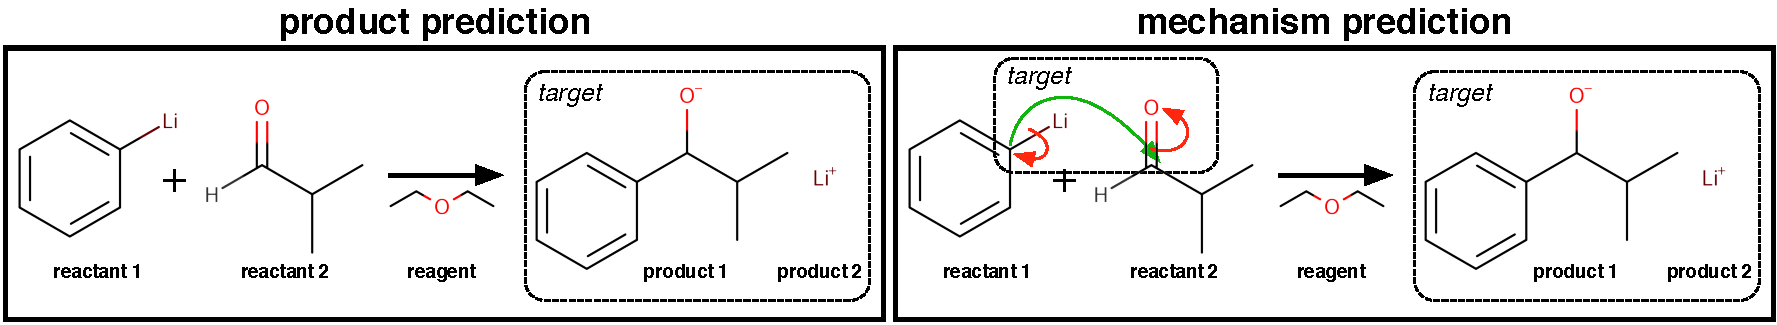
\includegraphics[width=\textwidth]{reaction_diagram}
\caption{Left: the reaction prediction problem: Given the reactants and reagents, predict the structure of the product. Right: the reaction mechanism prediction problem: Given the reactants, reagents and products, predict how the reaction occurred to form the products.}
\label{fig:task-overview}
\end{figure*}


Consider Figure \ref{fig:task-overview}. In it we show the two challenges we tackle in this paper. 
On the left we show reaction prediction; this involves predicting the reaction products, given a set of reactants and reagents. However, for this task we do not care {\em how} the reactants react.
 This job of finding the {\em how} is the target in reaction mechanism prediction, where the steps in a reaction are called a reaction mechanism.
 Before discussing how our model predicts mechanisms in the next section we use the rest of this section to describe the types of reactions we consider in this paper, and their properties.
%\todo[]{Where is the related work section going...? "And how it relates to previous work on reaction prediction. -- " }

\paragraph{Chemical reactions.}
%In reality, the structure of a molecule is due to how electrons on each atom are interacting with each other. 

%% Bond localization?
Molecules consist of a set of atoms that are arranged into a structure by a set of bonds. 
As such, molecules can be depicted as a graph structure, where each node is an atom and each edge is a bond.
Edges are only used to represent covalent bonds. 
These covalent bonds % \todo[]{Marwin is this right} 
represent the fact that one or more pairs of electrons are shared between the atoms that the bond connects. 
% Ionic bonds are bonds in which one atom completely borrows the electrons of another atom and the atoms become charged, however these are not represented by edges but rather by attaching charge to vertices in the graph \todo[]{do we really need this part about ionic bonds?}.

%Molecules are broken and built via reactions. 
Just as electrons describe the current structure of molecules, they also describe how molecules react with other molecules to produce new ones. 
All chemical reactions involve the movement of electrons along paths of atoms in a set of reactant molecules. 
This movement causes the formation and breaking of chemical bonds that changes the reactants into a new set of product molecules. 
%The movement occurs because it allows the set of molecules to move to a lower (and thus more favorable) energy state \todo[]{Marwin: is this right? Is this realted to exothermic and endothermic reactions}.
In this work, we will consider reactions that satisfy the following assumptions:
% \begin{enumerate}
% \item are single-step, so-called \emph{elementary} reactions.
% \item involve a pair of electrons, so-called \emph{heterolytic} reactions.
% \item either start with electrons on single atom, or with the electrons in an existing bond.
% \end{enumerate}
\begin{assumption}
Reactions are single-step\todo{MS:i am not sure this is really needed}, so-called \emph{elementary} reactions.
\label{assume:elem}
\end{assumption}

\begin{assumption}
Reactions involve pairs of electrons moving, so-called \emph{heterolytic} reactions.
\label{assume:het}
\end{assumption}

\begin{assumption}
Reactions either start with electrons on a single atom (called \emph{free electrons}), or with the electrons in an existing bond.
\label{assume:atom_bond}
\end{assumption}

These sorts of reactions describe 81\% of \emph{organic reactions}\cite{herges1994coarctate} \footnote{Organic reactions that do not satisfy these assumptions are homolytic reactions, and concerted reactions.}.
Organic reactions are those involving Carbon atoms, and have a large number of applications from drug design to the invention of new materials\cite{segler2018planning}.
Note that reactions which are multi-step can be decomposed into multiple single-step reactions in order to satisfy Assumption~\ref{assume:elem}.
%For this reason organic reactions has been the focus of recent work in reaction prediction in machine learning \cite{jin2017predicting,schwaller2017found}. 

\paragraph{Reactions as single electron paths.}
If reactions satisfy the above assumptions, then a chemical reaction is the result of pairs of electrons moving in a \emph{single path} through the reactant atoms. 
Further, this electron path will alternately remove existing bonds in molecules, and form new ones. We show this alternating structure in the right hand part of Figure \ref{fig:task-overview}. \todo[]{someone check the chemically accurateness of this.}
In this Figure, the reaction starts by taking the pair of electrons between the Li and C atoms and moving them to the C atom (step 1). This is a remove bond step. 
Next comes an add step where electrons are moved from the C atom to form a bond between the two reactant molecules (step 2).
Finally a pair of electrons are removed between a C and O and moved to the O atom, ending the reaction (step 3).

As a byproduct of predicting this series of electron steps we are also able to predict the final products.
However, there are a number of benefits of predicting electron paths over predicting the outcomes of reactions directly (as in previous work \cite{jin2017predicting,schwaller2017found}):
\begin{itemize}
\item \textbf{Easy to interpret}: If the model makes a mistake, it is easy to see where it goes wrong by comparing the steps of the path with the correct steps.
\item \textbf{Sparse}: Reactions often only affect between 3 and 7 atoms out of anywhere from 10-50 reactant atoms. Modeling the reaction as a path allows us to exploit this sparsity.
\item \textbf{Chemical constraints}: Learning a path allows us to easily incorporate chemical constraints, such as the alternating removal and addition of bonds, among others.
\item \textbf{Compositionally}: Learning to combine lower-level abstractions of chemistry potentially allows to generalize better.
\end{itemize}
The only other work we are aware of to use machine learning to predict reaction mechanism are the works \cite{kayala2011learning,kayala2012reactionpredictor}. However,
it relies on complex hand-coded rules and expert-annotated datasets, which are usually small and proprietary.
% Machine learning has been applied mostly for the quantum chemistry-level\cite{NIPS2012_4830,schutt2017schnet}. Additionally, various models have been proposed to predict global rewriting rules for reaction prediction\cite{coley2017prediction,jin2017predicting,neural-symbolic,schwaller2017found,wei2016neural,zhang2005structure}. These models can be trained on large sets of reported chemical reactions. 
%At the medium level of abstraction, Kayala et al. proposed a model to predict electron shift steps using of two independently learned learning-to-rank and scoring stages,
% which however relies on complex hand-coded rules and expert-annotated datasets, which are usually very small.

